\documentclass[,man]{apa6}
\usepackage{lmodern}
\usepackage{amssymb,amsmath}
\usepackage{ifxetex,ifluatex}
\usepackage{fixltx2e} % provides \textsubscript
\ifnum 0\ifxetex 1\fi\ifluatex 1\fi=0 % if pdftex
  \usepackage[T1]{fontenc}
  \usepackage[utf8]{inputenc}
\else % if luatex or xelatex
  \ifxetex
    \usepackage{mathspec}
  \else
    \usepackage{fontspec}
  \fi
  \defaultfontfeatures{Ligatures=TeX,Scale=MatchLowercase}
\fi
% use upquote if available, for straight quotes in verbatim environments
\IfFileExists{upquote.sty}{\usepackage{upquote}}{}
% use microtype if available
\IfFileExists{microtype.sty}{%
\usepackage{microtype}
\UseMicrotypeSet[protrusion]{basicmath} % disable protrusion for tt fonts
}{}
\usepackage{hyperref}
\hypersetup{unicode=true,
            pdftitle={nStreams Analysis},
            pdfauthor={Charles J. H. Ludowici~\& Alex O. Holcombe},
            pdfkeywords={keywords},
            pdfborder={0 0 0},
            breaklinks=true}
\urlstyle{same}  % don't use monospace font for urls
\usepackage{graphicx,grffile}
\makeatletter
\def\maxwidth{\ifdim\Gin@nat@width>\linewidth\linewidth\else\Gin@nat@width\fi}
\def\maxheight{\ifdim\Gin@nat@height>\textheight\textheight\else\Gin@nat@height\fi}
\makeatother
% Scale images if necessary, so that they will not overflow the page
% margins by default, and it is still possible to overwrite the defaults
% using explicit options in \includegraphics[width, height, ...]{}
\setkeys{Gin}{width=\maxwidth,height=\maxheight,keepaspectratio}
\IfFileExists{parskip.sty}{%
\usepackage{parskip}
}{% else
\setlength{\parindent}{0pt}
\setlength{\parskip}{6pt plus 2pt minus 1pt}
}
\setlength{\emergencystretch}{3em}  % prevent overfull lines
\providecommand{\tightlist}{%
  \setlength{\itemsep}{0pt}\setlength{\parskip}{0pt}}
\setcounter{secnumdepth}{0}
% Redefines (sub)paragraphs to behave more like sections
\ifx\paragraph\undefined\else
\let\oldparagraph\paragraph
\renewcommand{\paragraph}[1]{\oldparagraph{#1}\mbox{}}
\fi
\ifx\subparagraph\undefined\else
\let\oldsubparagraph\subparagraph
\renewcommand{\subparagraph}[1]{\oldsubparagraph{#1}\mbox{}}
\fi

%%% Use protect on footnotes to avoid problems with footnotes in titles
\let\rmarkdownfootnote\footnote%
\def\footnote{\protect\rmarkdownfootnote}


  \title{nStreams Analysis}
    \author{Charles J. H. Ludowici\textsuperscript{1}~\& Alex O.
Holcombe\textsuperscript{1}}
      \date{5/18/2017}

\shorttitle{SHORTTITLE}
\affiliation{
\vspace{0.5cm}
\textsuperscript{1} The University of Sydney}
\keywords{keywords\newline\indent Word count: X}
\usepackage{csquotes}
\usepackage{upgreek}
\captionsetup{font=singlespacing,justification=justified}

\usepackage{longtable}
\usepackage{lscape}
\usepackage{multirow}
\usepackage{tabularx}
\usepackage[flushleft]{threeparttable}
\usepackage{threeparttablex}

\newenvironment{lltable}{\begin{landscape}\begin{center}\begin{ThreePartTable}}{\end{ThreePartTable}\end{center}\end{landscape}}

\makeatletter
\newcommand\LastLTentrywidth{1em}
\newlength\longtablewidth
\setlength{\longtablewidth}{1in}
\newcommand{\getlongtablewidth}{\begingroup \ifcsname LT@\roman{LT@tables}\endcsname \global\longtablewidth=0pt \renewcommand{\LT@entry}[2]{\global\advance\longtablewidth by ##2\relax\gdef\LastLTentrywidth{##2}}\@nameuse{LT@\roman{LT@tables}} \fi \endgroup}


\DeclareDelayedFloatFlavor{ThreePartTable}{table}
\DeclareDelayedFloatFlavor{lltable}{table}
\DeclareDelayedFloatFlavor*{longtable}{table}
\makeatletter
\renewcommand{\efloat@iwrite}[1]{\immediate\expandafter\protected@write\csname efloat@post#1\endcsname{}}
\makeatother
\usepackage{lineno}

\linenumbers

\authornote{Add complete departmental affiliations for each
author here. Each new line herein must be indented, like this line.

Enter author note here.

Correspondence concerning this article should be addressed to Charles J.
H. Ludowici, USYD. E-mail:
\href{mailto:charles.ludowici@sydney.edu.au}{\nolinkurl{charles.ludowici@sydney.edu.au}}}

\abstract{
Enter abstract here. Each new line herein must be indented, like this
line.


}

\usepackage{amsthm}
\newtheorem{theorem}{Theorem}[section]
\newtheorem{lemma}{Lemma}[section]
\theoremstyle{definition}
\newtheorem{definition}{Definition}[section]
\newtheorem{corollary}{Corollary}[section]
\newtheorem{proposition}{Proposition}[section]
\theoremstyle{definition}
\newtheorem{example}{Example}[section]
\theoremstyle{definition}
\newtheorem{exercise}{Exercise}[section]
\theoremstyle{remark}
\newtheorem*{remark}{Remark}
\newtheorem*{solution}{Solution}
\begin{document}
\maketitle

The brain processes a stream of temporally noisy visual information.
Several factors affect the time it takes to process a visual signal.
These include: where it falls in the visual field (Poggel \&
Strasburger, 2004), its contrast (reference), its location relative to
the spatial locus of attention (Carrasco, 2011) and its location in time
relative to attentional events (D. E. Broadbent \& Broadbent, 1987; Dux
\& Marois, 2009). From this sea of noisy timing data, the brain must
sometimes determine when two events were simultaneous. How does this
happen? In this article, we investigate the temporal distribution of
percieved simultaneity between rapid events. To do so, we must use tasks
where participants select a particular event from a dynamic display.
Experiments using such tasks have highlighted two potential mechanisms
by which the brain may achieve this aim.

Attention, the ability to prioritise stimuli for visual processing based
on their kind or location, is one such mechanism. In tasks where there
is uncertainty about the position of the response-relevant event, such
as multiple stream RSVP (Goodbourn \& Holcombe, 2015a; Holcombe, Nguyen,
\& Goodbourn, 2017) or visual search (Nakayama \& Mackeben, 1989),
sudden stimulation at a peripheral location causes that location to be
prioritised relative to the rest of the visual field. This
prioritisation is evident in improved detection and identification
reaction times and contrast sensitivity at that location (see Carrasco,
2011 for a review). It is not under conscious control and is referred to
as \enquote{exogenous} to distinguish it from more willful
prioritisation (endogenous or feature-based attention). Attention
facilitates the selection of object features to produce a bound percept.
The most famous example of this is Treisman and Schmidt's (1982)
illusory conjunctions. They demonstrated that features are mislocated
when attention is overloaded in brief, static presentations. This
selection can occur in dynamic displays too. Holcombe and Cavanagh
(2008) presented participants with dot patterns that alternated between
moving away from and towards fixation at a rate of 2.66Hz. The patterns
changed colour from green to red at the same rate, but the latency
between colour and motion changes was varied. The transitions between
colours and motions were seen as simultaneous when the motion change
preceded the colour change, consistent with previous reports (Moutoussis
\& Zeki, 1997; Nishida \& Johnston, 2002), but this apparent lag in
processing disappeared when Holcombe and Cavanagh presented an exogenous
attention cue (a white ring) with the stimulus. Under this condition the
relative timing between colour and motion changes that best yielded
apparent synchrony was close to 0. In other words, the exogenous cue
allowed participants to correctly identify when colour and motion
changes were simultaneous.

This article is about temporal processing, so it is worth describing the
temporal properties of an exogenous attention shift. The selection of
any two events in time must happen after the onset of the cue, because
the shift is triggered by the cueing stimulus. The deployment of
exogenous attention seems to be most efficacious around 100-120ms after
the onset of the cue and then declines (Carrasco, 2011; Nakayama \&
Mackeben, 1989). The time at which attention arrives at the cued
position will be distributed with positive skew. The probability of
completing the shift at the time of the cue's onset is zero, because
this is the process that triggers the shift. The probability of
completing the shift then increases rapidly, and trails off in the same
manner that reaction times are distributed. This skew comes about
because the process has a lower bound at the time of the cue, but no
upper bound (apparently something in the Luce RT book about this) The
effect of an exogenous cue on accuracy in visual search tasks yields a
distribution with this shape (Nakayama \& MacKeben, 1983). Our task
{[}which I haven't explained yet{]} provides a measure of the arrival
time of attention because the first item to be percieved is the item
selected. The accuracy pattern in static tasks where SOA is varied, on
the other hand, reflects arrival times and the overlap between the
application of attention and the stimulus. Note that because we are
concerned with selection of an event from a dynamic display, for events
briefer than 100ms, the probability of selecting that event from the
visual stream is low. Any distribution of selection times produced by an
attention shift will thus have positive skew and be entirely post-cue.

\begin{figure}
\centering
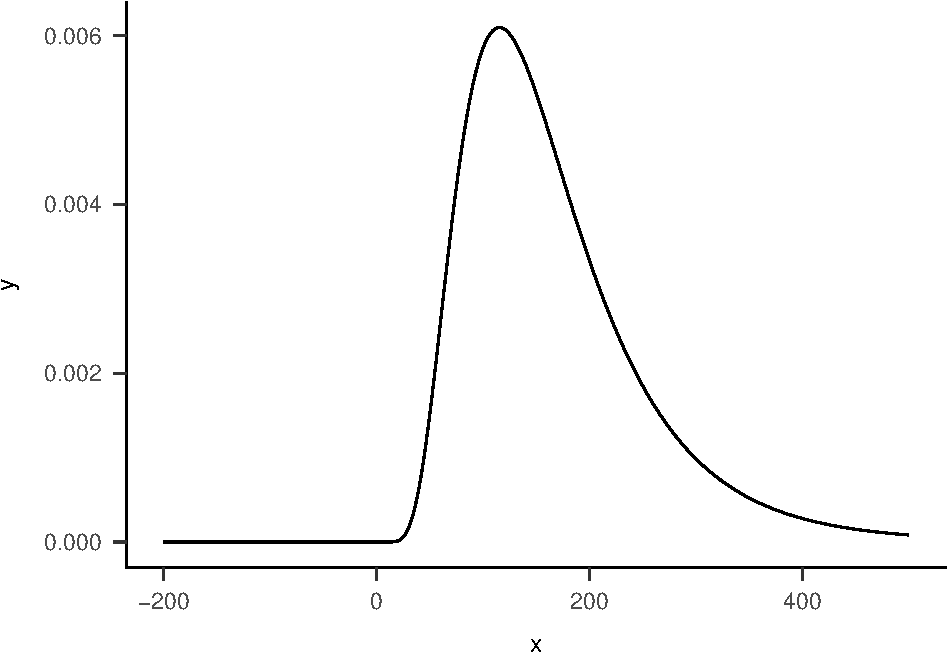
\includegraphics{nStreams_Bayesian_files/figure-latex/unnamed-chunk-2-1.pdf}
\caption{}
\end{figure}

Goodbourn and Holcombe (2015b) propose that rapidly decaying buffer of
visual information may be another source of information for judging
simultaneity. This buffer contains decaying representations of visual
events.Unlike the attention shift there is no triggering process. The
buffer is always recording events. One item from the buffer is selected
for tokenisation and subsequent consolidation into working memory. This
is based on some task-relevant factor such as simultaneity with a cue.
Goodbourn and Holcombe (2015b) argued for the presence of this storage
based on RSVP data. In each trial of their experiments participants saw
2 RSVP streams containing letters in a random order with no repeats. One
or both of the streams were cued at one point on each trial with white
ring. Participants were tasked with reporting the cued letter(s). The
lack of repeats allowed Goodbourn and Holcombe (2015b) to map each
response onto a point in time based on where that letter appeared in the
relevant stream and build a temporal distribution of responses. After
accounting for guessing (details in Modelling below), Goodbourn and
Holcombe (2015b) found that there were nonguessing responses from at the
cue or before, despite the fact the cue was a white circle with a rapid
onset, exactly the sort of stimulus we would expect to elicit an
exogenous attention shift. These responses are impossible under an
attention shift account, however they are possible if the process that
selects an item for conslidation is error prone and operates over item
representations from timepoints that preceded the the cue.

The Goodbourn and Holcombe (2015b) buffer is a brief, high-capacity
store of visual information, similar to iconic memory (IM; Sperling,
1960) and fragile memory (Sligte, Scholte, \& Lamme, 2008). However, it
is not either of these kinds of memory. IM is a was proposed based on
experiments showing that a cue presented after the offset of a brief
visual array indicating a part of the array for report produces better
memory for the array than without the cue. The cued information is
thought to be selected from IM and sustained while the unselected
information decays. Recently, another form of visual memory has been
demonstrated using these cues at different timescales. This memory
operates at a timepoint beyond the decay of IM and is not masked in the
same way as IM (Pinto, Sligte, Shapiro, \& Lamme, 2013; Sligte et al.,
2008, but see Matsukura \& Hollingworth, 2011 for a dissenting opinion).
Iconic memory is extremely sensitive to masking from any stimulation at
the visual location of the array. FM is not sensitive to masking from
just any stimulation, but is masked by objects of the same kind at the
visual location of the array (Pinto et al., 2013). Goodbourn and
Holcombe (2015b) used RSVP, where subsequent items - all of one kind -
mask previous items. Under these conditions it is not possible to use IM
or FM to perform the task.

The current article uses multiple-stream RSVP investigate the temporal
properties of Goodbourn and Holcombe (2015b)'s bufferas we manipulate
the buffer's workload. We look for evidence of attention shifts in our
data and in the initial Goodbourn and Holcombe (2015b) data. The
capacity of the buffer is unknown, as Goodbourn and Holcombe (2015b)
used a maximum of 2 RSVP streams. We increased the number of streams to
8, because this should exceed the buffer's capacity. We predicted under
these conditions participants would rely on attention shifts rather than
to select items from the cued stream. This strategy would produce a
temporal distribution of responses that is positively skewed and
entirely post-cue, whereas using buffered information for the task will
create a normal distribution of responses that include timepoints from
at the cue or before. We fit models corresponding to both these
scenarios to detect the different strategies and interpret the estimated
parameters of these models to draw inferences about the temporal
properties of visual processing under these conditions.

\subsection{Modelling}\label{modelling}

Our modelling is based on the temporal distribution of responses over
many trials. We match each trial's response to a particular point in
time on that trial - its serial position error (SPE). We fit
distributions to the distributions of SPEs from all trials of a
particular condition. The empirical RSVP distributions are thought to be
a mixture of two components. One is a uniform component corresponding to
trials in which the participant made a guess about the identity of the
cued letter. The other component of the distribution will be responses
informed by the cue. These do not have to be accurate responses.
Instead, they can reflect the variance of a temporal binding process,
the items selected after an attention shift, or some other process.
Attention shifts and buffering predict different non-guessing
distributions for the SPE distribution. If the task is performed using
information from a buffer, we would expect a Gaussian distribution that
includes items from at the cue or before, because the buffer may
erroenously select items from before the cue as coincident with it.
Goodbourn and Holcombe (2015b) used this latter mixture to model their
data, we refer to it as the buffering model.

If, on the other hand, participants select items from the cued stream
using an attention shift, the SPE distribution will have a positively
skewed non-guessing component. An attention shift will not trigger until
the cue is detected. Thus, we expect the non-guessing component to not
include any responses from before the cue and to have positive skew. To
model this, we use the log-normal distribution as the non-guessing
distribution. The log-normal is a positively-skewed distribution that is
only defined for values greater than 0.\footnote{Update: My initial
  reasoning was that our items would be too brief for the correct item
  to be selected by an attention shift, but I no longer think this is
  the case. The lognormal might not be the best distribution for our
  purposes here.} This distribution thus has the skew and domain
associated with an attention shift.

We fit both these models and compared them using Bayes factors. Each
participant produced a distribution of SPEs in each condition and we fit
the models to each of these distributions. We computed Bayes factors
from the Bayesian Information Criterion for each model fit (Wagenmakers,
2007). These Bayes factors are used to select the best fitting model.

\section{Methods}\label{methods}

\subsection{Participants}\label{participants}

10 naive participants took part in the study in exchange for course
credit.

\subsection{Apparatus}\label{apparatus}

The experiment was controlled by a Macbook Pro running Mac OSX 10.8.5
and was programmed in Python 2.7.12 using Psychopy. Stimuli were
presented on a Mitsubishi Diamond Pro 2070SB with a resolution of 1024 x
768 pixels and a refresh rate of 60Hz. Participants viewed the
experiment from a distance of 57cm. To ensure that they did not break
fixation, participants' right eye movements were tracked with an SR
Research Eyelink 1000.

\section{2 vs 8 Streams}\label{vs-8-streams}

\subsection{Latency Analyses}\label{latency-analyses}

\begin{figure}
\centering
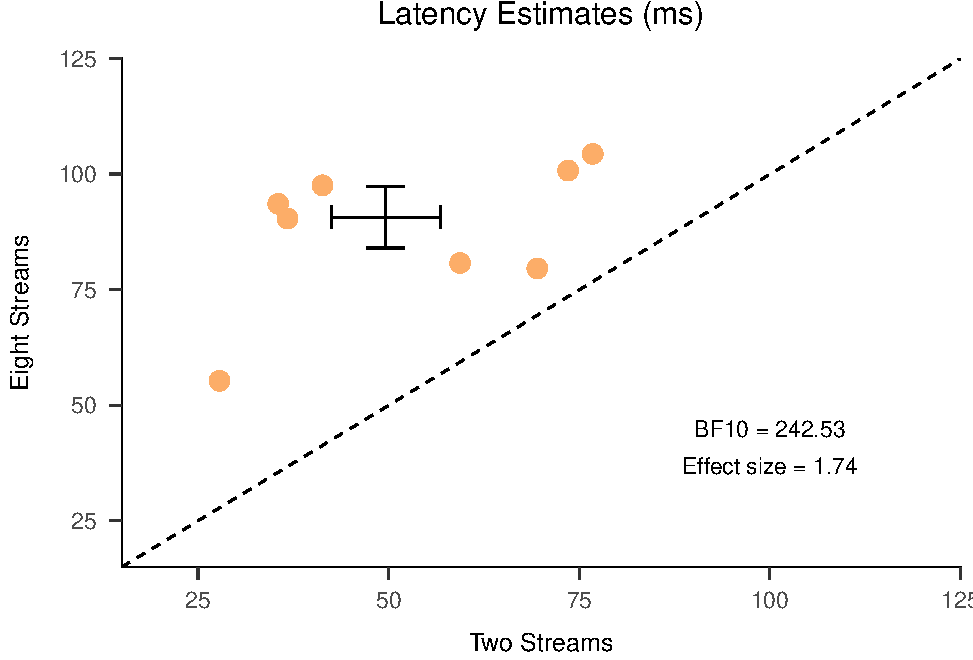
\includegraphics{nStreams_Bayesian_files/figure-latex/unnamed-chunk-3-1.pdf}
\caption{}
\end{figure}

BF\textsubscript{10} is 242.53. There is strong evidence for a
difference in mean latency between the two- and eight-streams
conditions. Mean latency for the two-streams condition (M = 49.62, SD =
22.55) is less than the mean latency for the eight-streams condition (M
= 90.61, SD = 20.98).

The nonguessing distribution is delayed in the eight-streams relative to
the two-streams condition. There appears to be some cost for increasing
the number of streams. Two possible reasons for this are: an attentional
cost for distributing attention over more visual space, or a cost of
interference due to the increased number of items. These possibilities
are theories used in the visual search literature to explain set-size
effects (i.e. Palmer, 1994). This literature distinguished between
perceptual effects and those that were due to attention. These theories
were tested by holding the number of items constant - thus controling
any perceptual effects - but cueing a number of positions as potential
target locations. Support for an attentional effect is manifest whenever
the effect of set size is similar to that of the pre-cueing
manipulation.

\subsection{Precision Analysis}\label{precision-analysis}

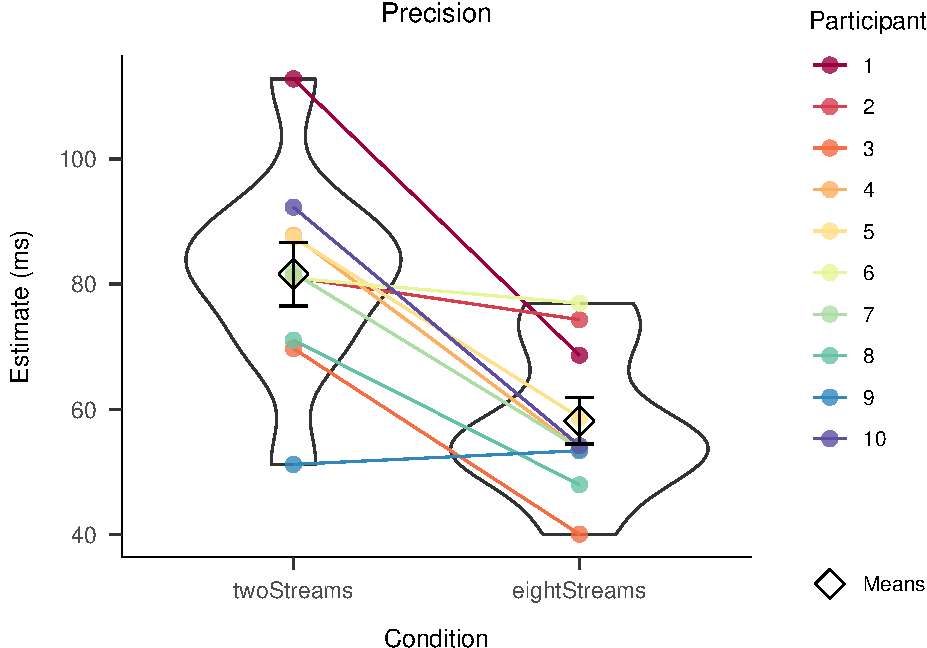
\includegraphics{nStreams_Bayesian_files/figure-latex/unnamed-chunk-4-1.pdf}
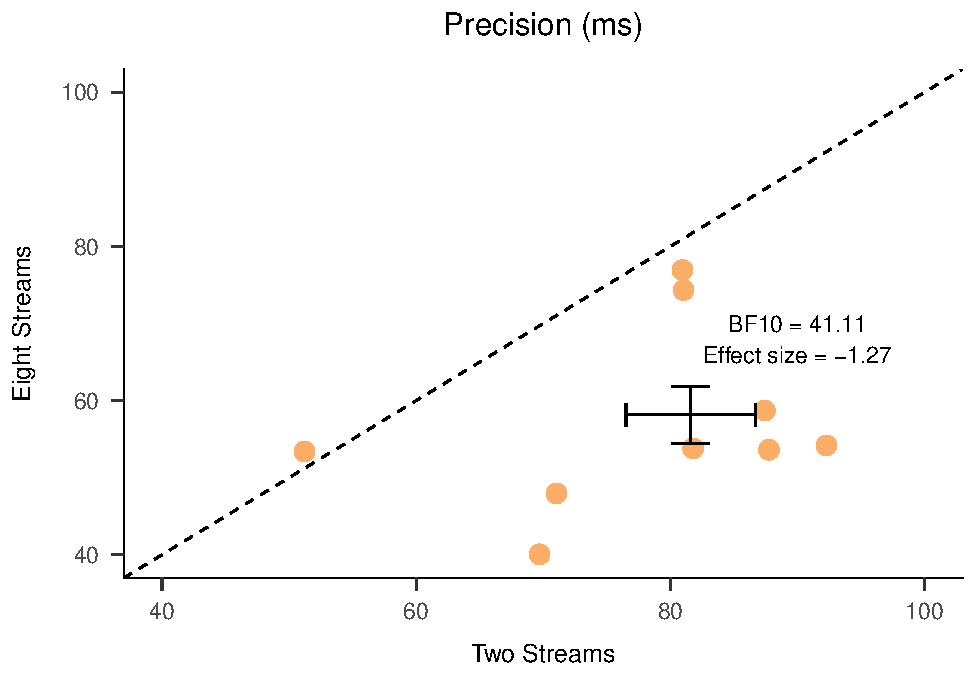
\includegraphics{nStreams_Bayesian_files/figure-latex/unnamed-chunk-4-2.pdf}

Strangely, the precision of the nonguessing distribution decreases as
the number of streams increases. The two-streams condition (M = 81.60,
SD = 16.11) has more variance in the nonguessing distributions than the
eight-streams conditions (M = 58.16, SD = 11.71; BF\textsubscript{10} =
41.11). In a buffering account this could be because as the number of
simultaneous items increases there is less capacity to store
non-simultaneous items. In an attention shift account this is harder to
account for. One possible reason could be that an inability to spread
attention over eight streams causes participants to rely on only
exogenous attention - rather than an endo-exo mix - and the precision
we're seeing here reflects the variability in arrival times for
exogenous attention (check the ERP and behavioural literature for
exogenous attention estimates). Again, a pre-cuing manipulation is a
method for testing this hypothesis.

\subsection{Efficacy Analysis}\label{efficacy-analysis}

\begin{verbatim}
## [1] 0.3755812
\end{verbatim}

\begin{verbatim}
## [1] 0.5468815
\end{verbatim}

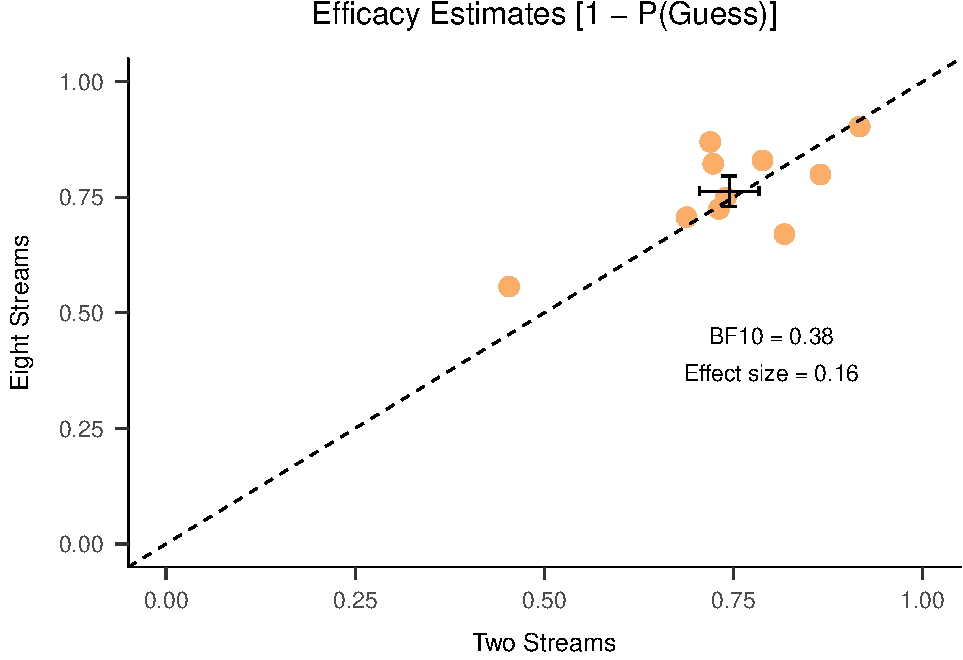
\includegraphics{nStreams_Bayesian_files/figure-latex/unnamed-chunk-5-1.pdf}
The Bayesian analysis for the efficacy data shows weak evidence for a
lack of an effect (BF\textsubscript{10} = 0.38). The mean for the
two-streams condition is 0.74 (SD = 0.12). The mean for the
eight-streams condition is 0.76 (SD = 0.10).
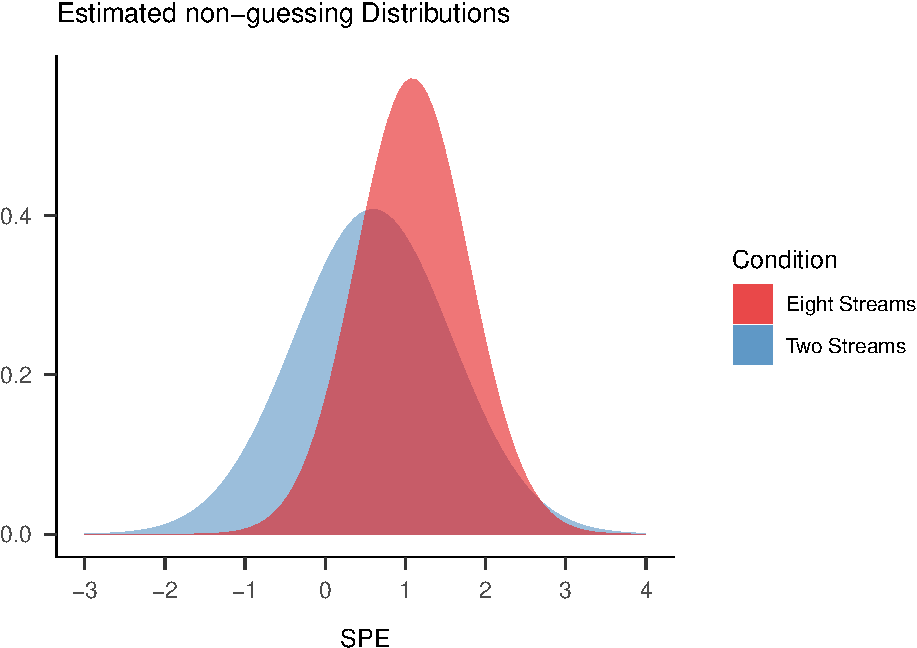
\includegraphics{nStreams_Bayesian_files/figure-latex/unnamed-chunk-6-1.pdf}

\section{Precue Data}\label{precue-data}

\begin{verbatim}
## 
##  Paired t-test
## 
## data:  preCueLatency$eightStreams and preCueLatency$twoStreams
## t = 3.9875, df = 12, p-value = 0.001802
## alternative hypothesis: true difference in means is not equal to 0
## 95 percent confidence interval:
##  10.55607 35.98837
## sample estimates:
## mean of the differences 
##                23.27222
\end{verbatim}

In this experiment, the program presented 8 streams on each trial. Prior
to the onset of a trial, participants saw a circular array of hashmarks
for 250ms, as in Goodbourn and Holcombe (2015b), this was followed by a
blank screen for 500ms, a fixation point for 1000ms and then the RSVP
streams. The possible position of the cue on a trial was indicated by
white rings around either two or eight streams. These mimicked the
position of the streams in the first experiment's conditions. This
experiment tests whether any differences between the two or eight
streams conditions are due to increasing interference that scales with
the number of streams - this theory predicts no difference between
conditions in this experiment - or due to a cost involved in spreading
attention over a larger area of visual space - this theory predicts a
replication of the initial experiment's effects.

\subsection{Latency Analyses}\label{latency-analyses-1}

\begin{figure}
\centering
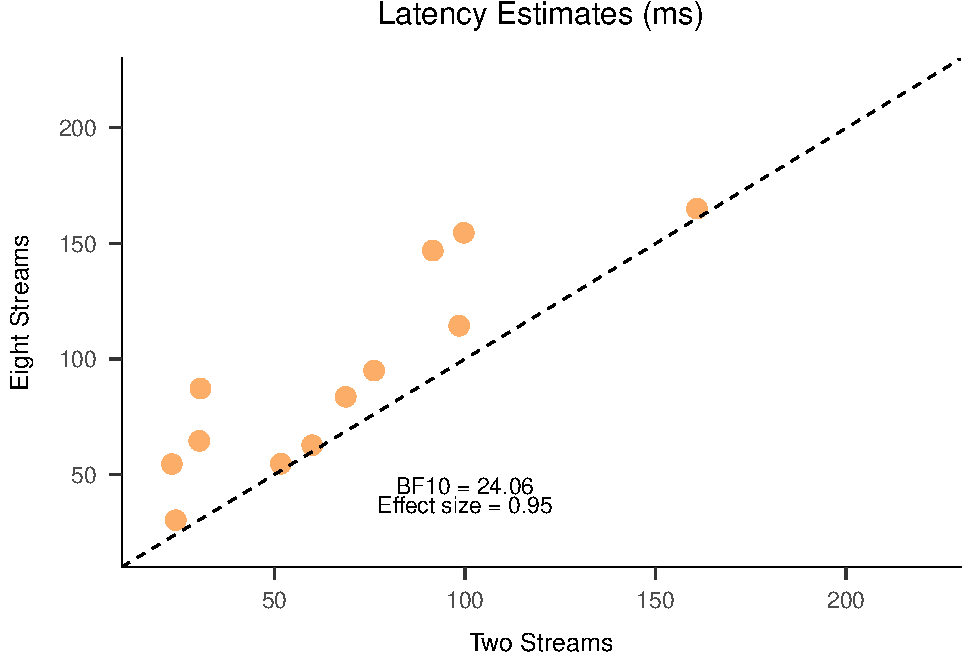
\includegraphics{nStreams_Bayesian_files/figure-latex/unnamed-chunk-8-1.pdf}
\caption{}
\end{figure}

The latency for the two-precues condition (M = 84.84, SD = 72.35) is
less than that of the eight-precues condition (M = 108.12, SD = 69.37;
BF\textsubscript{10} = 24.06).

\section{Precision Analysis}\label{precision-analysis-1}

\begin{verbatim}
## [1] 0.3467804
\end{verbatim}

\begin{verbatim}
## [1] 0.1791612
\end{verbatim}

\begin{figure}
\centering
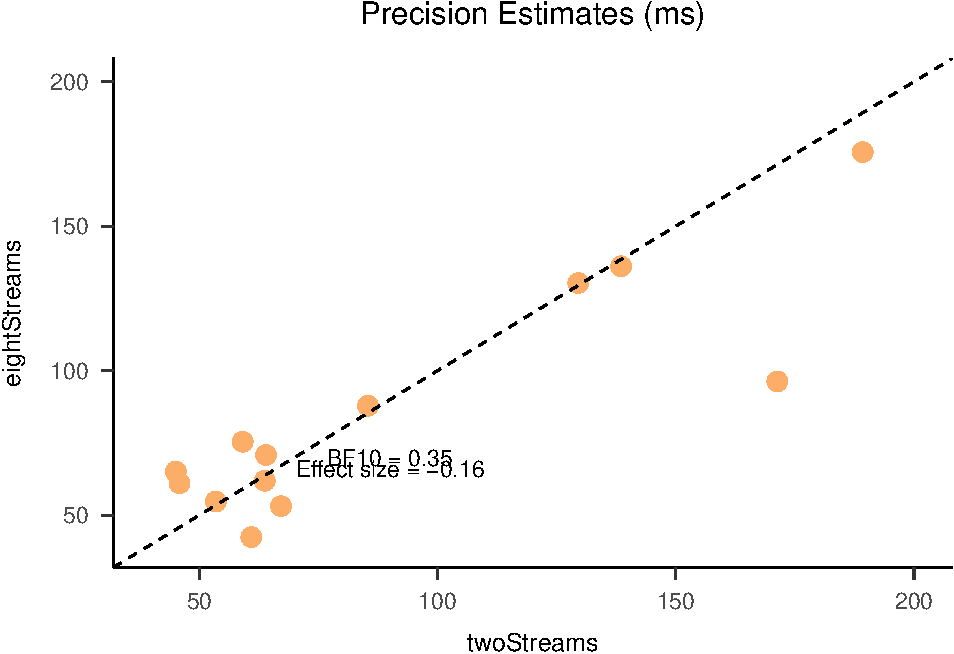
\includegraphics{nStreams_Bayesian_files/figure-latex/unnamed-chunk-9-1.pdf}
\caption{}
\end{figure}

There is weak evidence for no difference between the two conditions,
BF\textsubscript{10} = 0.35. The two-precues condition has a mean of
90.25 (SD = 49.49). The eight-precues condition has a mean of 85.46 (SD
= 39.31).

\section{Efficacy Analysis}\label{efficacy-analysis-1}

\begin{verbatim}
## [1] 0.7606536
\end{verbatim}

\begin{verbatim}
## [1] 0.1260706
\end{verbatim}

\begin{figure}
\centering
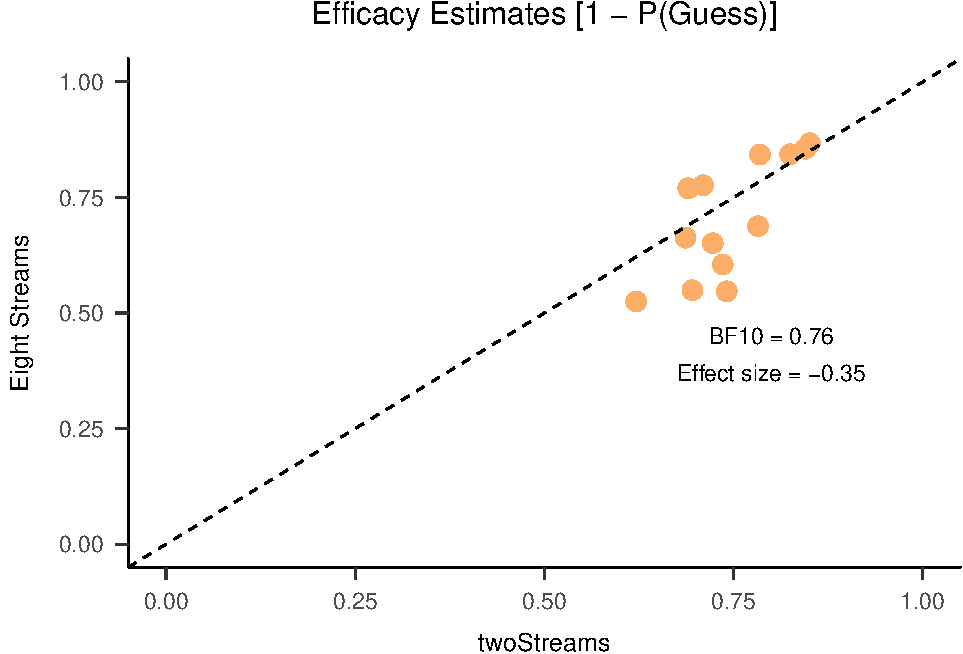
\includegraphics{nStreams_Bayesian_files/figure-latex/unnamed-chunk-10-1.pdf}
\caption{}
\end{figure}

There is weak evidence for no difference between the two conditions,
BF\textsubscript{10} = 0.76. The two-precues condition has a mean of
0.75 (SD = 0.07). The eight-precues condition has a mean of 0.71 (SD =
0.13).

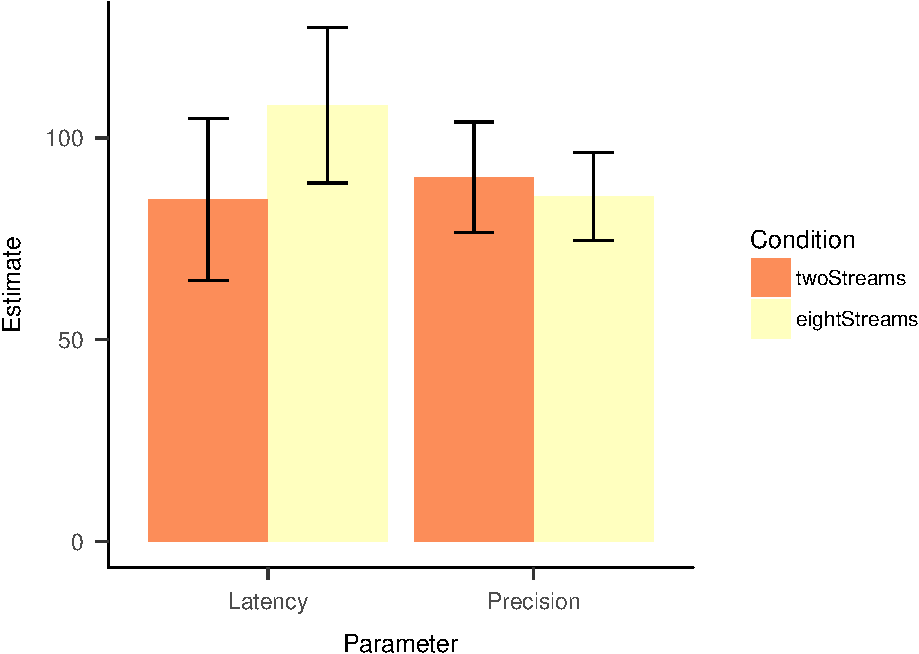
\includegraphics{nStreams_Bayesian_files/figure-latex/unnamed-chunk-11-1.pdf}
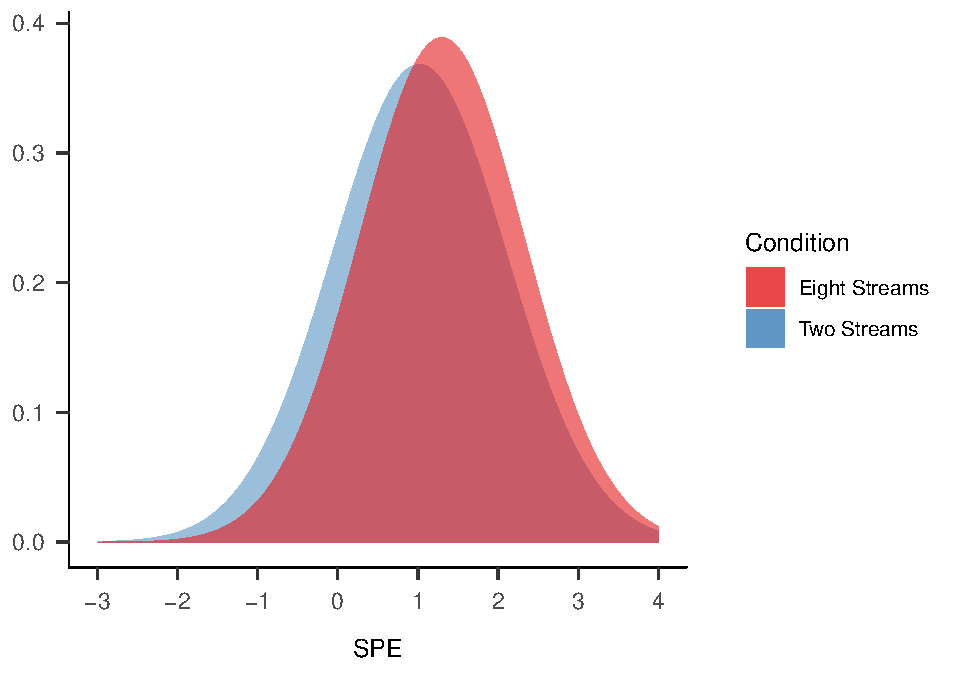
\includegraphics{nStreams_Bayesian_files/figure-latex/unnamed-chunk-11-2.pdf}

\subsection{Summary}\label{summary}

We replicated the effect of the number of streams on latency but not
precision in this experiment. The delayed latency in the eight-precue
condition relative to the two-precue condition cannot be because of
crowding-like interference due to the number of streams displayed
because the number of streams is constant across conditions. What
changes is the number of potential cue positions, and thus the number of
streams that must be monitored. Our latency results are then consistent
with the idea that monitoring several locations for a target is taxing
for the visual system and either the detection of the target or the
selection of items contingent on the target lag because of this.

\begin{verbatim}
## Bayes factor analysis
## --------------
## [1] Alt., r=0.707 : 0.3893135 ±0%
## 
## Against denominator:
##   Null, mu1-mu2 = 0 
## ---
## Bayes factor type: BFindepSample, JZS
\end{verbatim}

Palmer (1994) argues that pre-cueing components of a visual array while
holding the stimuli constant gives a measure of attentional
contributions to an effect. The results of our pre-cue experiment thus
suggest that the latency effect is due to an attentional effect. One
candidate is a cost associated with monitoring multiple stream
locations. In Hogendoorn, Carlson, Vanrullen, and Verstraten (2010) (and
Huang \& Pashler, which I haven't yet read), the authors distinguish
between attention's ability to optimise - i.e.~speed up - processing at
attended sites and its ability to select features and bind them into an
object. Precuing a stimulus manipulates monitoring - processing of the
cue should be sped up. However a bayesian t-test of the difference in
latencies between experiments in the two streams conditions yields only
weak evidence, and this evidence is in favour of the null (0.39).

\hypertarget{refs}{}
\hypertarget{ref-broadbent_detection_1987}{}
Broadbent, D. E., \& Broadbent, M. H. (1987). From detection to
identification: Response to multiple targets in rapid serial visual
presentation. \emph{Perception \& Psychophysics}, \emph{42}(2),
105--113.

\hypertarget{ref-carrasco_visual_2011}{}
Carrasco, M. (2011). Visual attention: The past 25 years. \emph{Vision
Research}, \emph{51}(13), 1484--1525.
doi:\href{https://doi.org/10.1016/j.visres.2011.04.012}{10.1016/j.visres.2011.04.012}

\hypertarget{ref-dux_attentional_2009}{}
Dux, P. E., \& Marois, R. (2009). The attentional blink: A review of
data and theory. \emph{Attention, Perception, \& Psychophysics},
\emph{71}(8), 1683--1700.

\hypertarget{ref-goodbourn_pseudoextinction_2015}{}
Goodbourn, P. T., \& Holcombe, A. O. (2015a). ``Pseudoextinction'':
Asymmetries in simultaneous attentional selection. \emph{Journal of
Experimental Psychology: Human Perception and Performance},
\emph{41}(2), 364. Retrieved from
\url{http://psycnet.apa.org/journals/xhp/41/2/364/}

\hypertarget{ref-goodbourn_pseudoextinction}{}
Goodbourn, P. T., \& Holcombe, A. O. (2015b). ``Pseudoextinction'':
Asymmetries in simultaneous attentional selection. \emph{Journal of
Experimental Psychology: Human Perception and Performance},
\emph{41}(2), 364. Retrieved from
\url{http://psycnet.apa.org/journals/xhp/41/2/364/}

\hypertarget{ref-hogendoorn_timing_2010}{}
Hogendoorn, H., Carlson, T. A., Vanrullen, R., \& Verstraten, F. A.
(2010). Timing divided attention. \emph{Attention, Perception, \&
Psychophysics}, \emph{72}(8), 2059--2068.

\hypertarget{ref-holcombe_implied_2017}{}
Holcombe, A. O., Nguyen, E. H., \& Goodbourn, P. T. (2017). Implied
reading direction and prioritization of letter encoding. \emph{Journal
of Experimental Psychology: General}, \emph{146}(10), 1420.

\hypertarget{ref-matsukura_does_2011}{}
Matsukura, M., \& Hollingworth, A. (2011). Does visual short-term memory
have a high-capacity stage? \emph{Psychonomic Bulletin \& Review},
\emph{18}(6), 1098--1104.
doi:\href{https://doi.org/10.3758/s13423-011-0153-2}{10.3758/s13423-011-0153-2}

\hypertarget{ref-nakayama_sustained_1989}{}
Nakayama, K., \& Mackeben, M. (1989). Sustained and transient components
of focal visual attention. \emph{Vision Research}, \emph{29}(11),
1631--1647. Retrieved from
\url{http://www.sciencedirect.com/science/article/pii/0042698989901442}

\hypertarget{ref-palmer_set-size_1994}{}
Palmer, J. (1994). Set-size effects in visual search: The effect of
attention is independent of the stimulus for simple tasks. \emph{Vision
Research}, \emph{34}(13), 1703--1721.
doi:\href{https://doi.org/10.1016/0042-6989(94)90128-7}{10.1016/0042-6989(94)90128-7}

\hypertarget{ref-pinto_fragile_2013}{}
Pinto, Y., Sligte, I. G., Shapiro, K. L., \& Lamme, V. A. (2013).
Fragile visual short-term memory is an object-based and
location-specific store. \emph{Psychonomic Bulletin \& Review},
\emph{20}(4), 732--739. Retrieved from
\url{http://link.springer.com/article/10.3758/s13423-013-0393-4}

\hypertarget{ref-poggel_visual_2004}{}
Poggel, D. A., \& Strasburger, H. (2004). Visual perception in space and
time-mapping the visual field of temporal resolution. \emph{Acta
Neurobiologiae Experimentalis}, \emph{64}(3), 427--437.

\hypertarget{ref-sligte_are_2008}{}
Sligte, I. G., Scholte, H. S., \& Lamme, V. A. F. (2008). Are There
Multiple Visual Short-Term Memory Stores? \emph{PLOS ONE}, \emph{3}(2),
e1699.
doi:\href{https://doi.org/10.1371/journal.pone.0001699}{10.1371/journal.pone.0001699}

\hypertarget{ref-sperling_information_1960}{}
Sperling, G. (1960). The information available in brief visual
presentations. \emph{Psychological Monographs: General and Applied},
\emph{74}(11), 1. Retrieved from
\url{http://psycnet.apa.org/journals/mon/74/11/1/}

\hypertarget{ref-wagenmakers_practical_2007}{}
Wagenmakers, E.-J. (2007). A practical solution to the pervasive
problems ofp values. \emph{Psychonomic Bulletin \& Review},
\emph{14}(5), 779--804.
doi:\href{https://doi.org/10.3758/BF03194105}{10.3758/BF03194105}


\end{document}
